\documentclass{article}
\usepackage[spanish]{babel}
	\deactivatetilden
\spanishdecimal{.}
\addto\captionsspanish{\def\tablename{Tabla}}
\addto\captionsspanish{\def\listtablename{\'Indice de tablas}}
\usepackage[numbers,sort&compress]{natbib}
\usepackage[T1]{fontenc}
\usepackage[utf8]{inputenc}
\usepackage{graphicx}
\usepackage{url}
\usepackage{graphicx}
\graphicspath{{Figuras/}}
\usepackage[numbers,sort&compress]{natbib}
\usepackage[clearempty,pagestyles]{titlesec}
\usepackage{anysize}
\usepackage{xcolor, colortbl}
\usepackage{array, multirow, multicol}
\usepackage{enumerate} 

\def\baselinestretch{1.5}
\papersize{27.9cm}{21.5cm} 
\marginsize{2cm}{2cm}{1cm}{1cm}

\title {Modelo de Urnas}
\author{Julio Garc\'ia}
\pagestyle{empty}

\pagestyle{empty}
\begin{document}
	\renewcommand{\listtablename}{Índice de tablas}
	\renewcommand{\tablename}{Cuadro}
	\maketitle
	
	\section{Introducción}
	En el presente trabajo se busca como objetivo principal el determinar un porcentaje de partículas que se podría filtrar dado un tamaño critico $C$, tomando en cuenta variaciones en tiempo ($t$), cantidad de partículas ($n$) y en valores creados ($k$) a partir de distribución normal para normalizarlos y convertirlos en cúmulos iniciales que suman $n$.  
                                                
	\section{Desarrollo}                                    
	En este trabajo se realiza experimentación variando valores de $t$, $k$ y $n$ (antes mencionados) para ver el efecto que tienen en un modelo de urnas en el que una cumulo de partículas puede ser filtrado solamente si su tamaño excede un valor crítico $C$.
	                                                        
	\section{Experimentación y resultados}                  
	En esta sección se describe el ambiente computacional y los resultados obtenidos con la simulación. El código de dicha simulación fue realizado en el lenguaje computacional Python en una computadora personal con procesador 1 Intel Core i7, con memoria RAM de 16GB y hasta 8 núcleos de procesamiento. Dicho código fue incorporado en el repositorio \cite{p_8}.  Se tomó como base el código de la Dra. Elisa Schaeffer \cite{p8}, en el que se realizaron las variaciones requeridas.
	
	A continuación, se presentan imágenes obtenidas.
	\newpage
	
		\begin{figure}[h!]
		\centering
		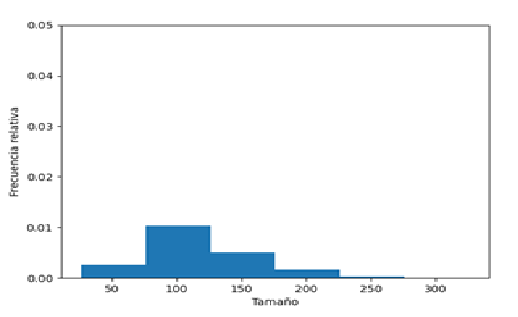
\includegraphics[width=0.7\linewidth]{Imagen_1.png}
		\caption{Paso 3 con ambos fenómenos}
		\label{fig:imagen1}
     	\end{figure}
     
	Cabe mencionar que se realizaron tres experimentos diferentes para cada valor de k, n seleccionado. Dichos valores están en el título de las gráficas  presentadas a continuación, por una parte se presentan diagramas de lineas  para respaldar el hecho de que el tiempo en el que se filtren las partículas parece no tener algún efecto en la proporción de partículas efectivamente filtradas. 
		\newpage
		
		\begin{figure}[h!]
		\centering
		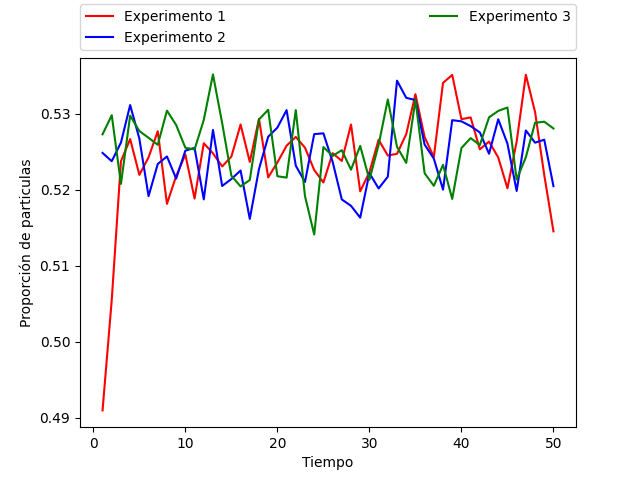
\includegraphics[width=0.5\linewidth]{Figure_1.png}
		\caption{Proporción de particulas filtradas: k=10000,n=1000000}
		\label{fig:imagen2}
		
		
		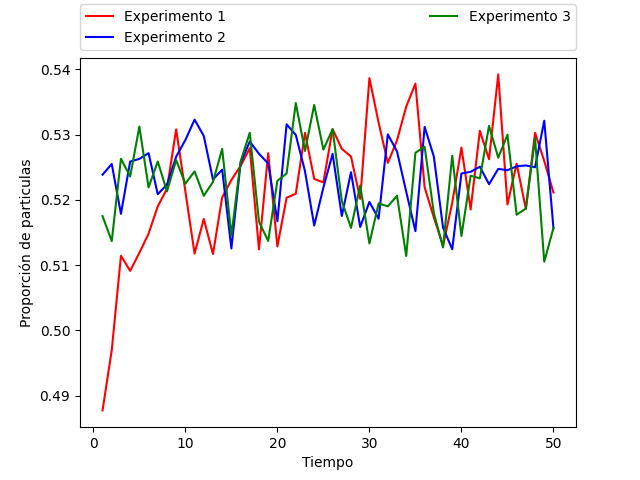
\includegraphics[width=0.5\linewidth]{Figure_2.png}
		\caption{Proporción de particulas filtradas: k=5000,n=1000000}
		\label{fig:imagen3}
		
	
		\end{figure}

		\newpage
	\begin{figure}[h!]
				\centering
	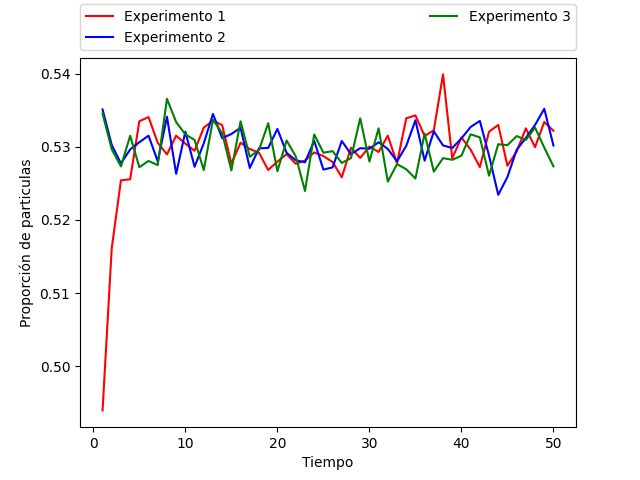
\includegraphics[width=0.5\linewidth]{Figure_3.png}
	\caption{Proporción de particulas filtradas: k=20000,n=1000000}
	\label{fig:imagen4}

	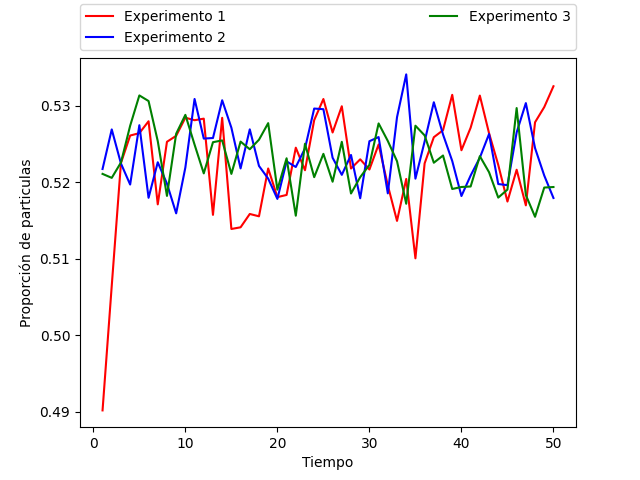
\includegraphics[width=0.5\linewidth]{Figure_4.png}
	\caption{Proporción de particulas filtradas: k=10000,n=2000000}
	\label{fig:imagen5}

	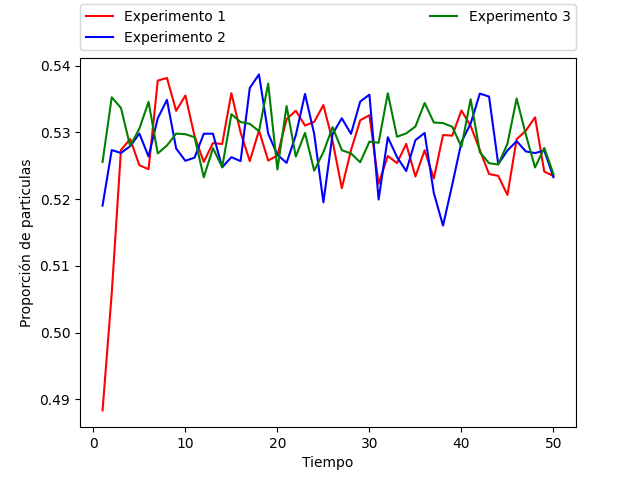
\includegraphics[width=0.5\linewidth]{Figure_5.png}
	\caption{Proporción de particulas filtradas: k=10000,n=500000}
	\label{fig:imagen6}
	
\end{figure}

Además se presentan a continuación diagramas de cajas y bigotes para verificar si podría haber diferencia entre una corrida y otra, fijando los valores para k,n. Con los siguientes diagramas podemos ver que no hay mucha diferencia entre un experimento y otro, con lo que podemos decir que el filtrado de particulas es mas o menos estable.

Además de que, al parecer, la variación de los valores de n,k tampoco afectan tanto al filtrado de partículas, ya que en todos los experimentos, sin importar la k, n se filtra en promedio un $52 \%$ de las partículas. Además de que con los diagramas radiales parece que el tiempo en el que se filtre tampoco tiene efecto.\\	
\newpage


	
\begin{figure}[h!]
	\centering
	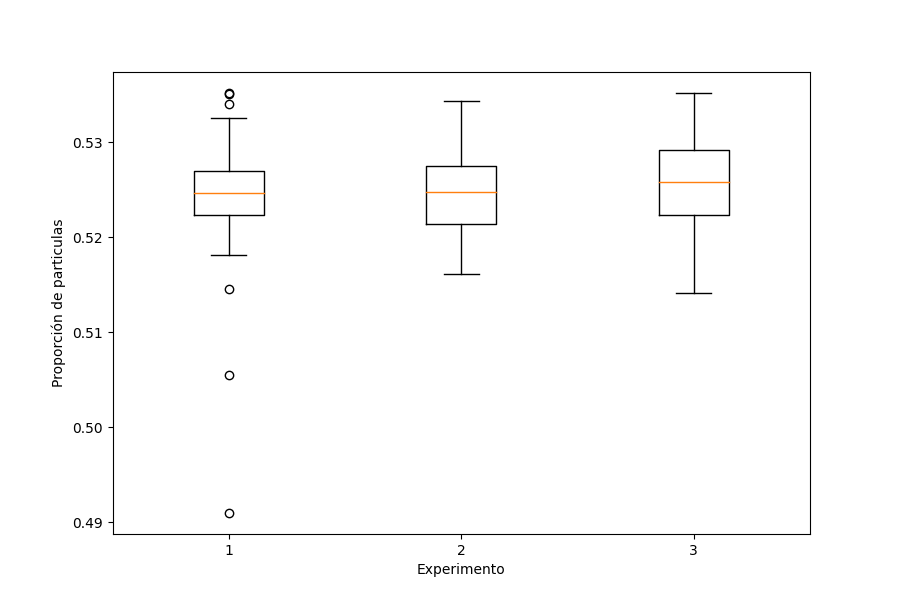
\includegraphics[width=0.5\linewidth]{bx_1.png}
	\caption{Proporción de particulas filtradas: k=10000,n=1000000}
	\label{fig:bx2}
	
	
	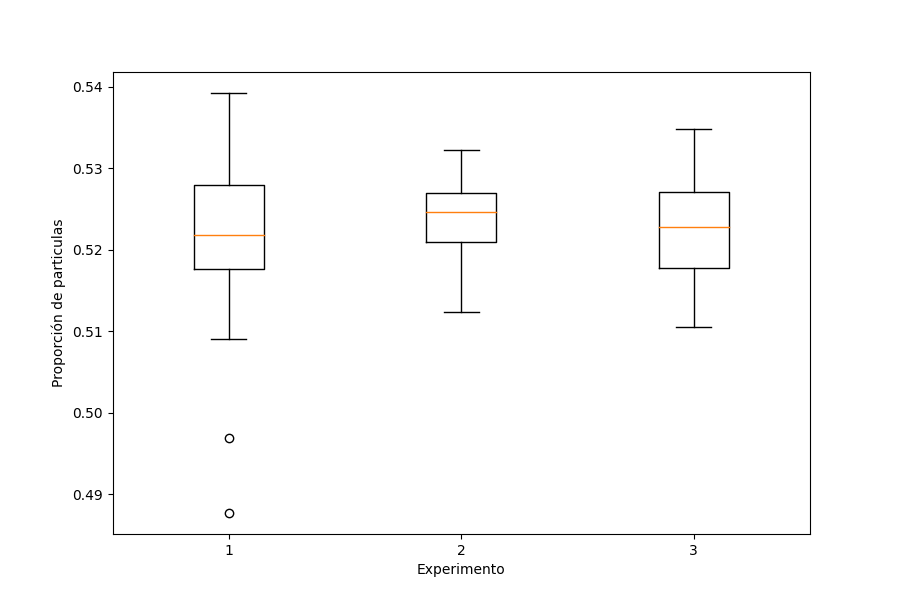
\includegraphics[width=0.5\linewidth]{bx_2.png}
	\caption{Proporción de particulas filtradas: k=5000,n=1000000}
	\label{fig:bx3}
	
	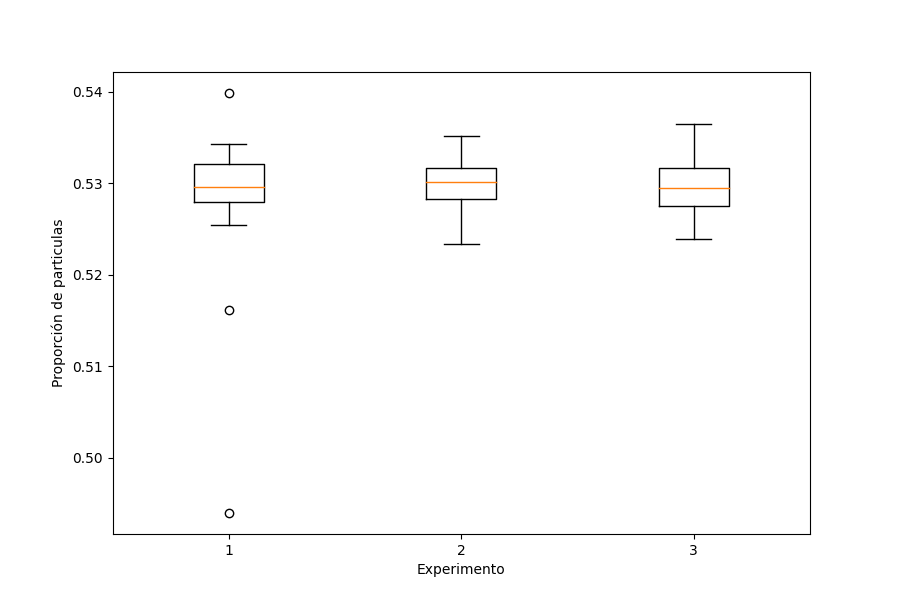
\includegraphics[width=0.5\linewidth]{bx_3.png}
	\caption{Proporción de particulas filtradas: k=20000,n=1000000}
	\label{fig:bx4}
	
\end{figure}

\newpage
\begin{figure}[h!]
	\centering
	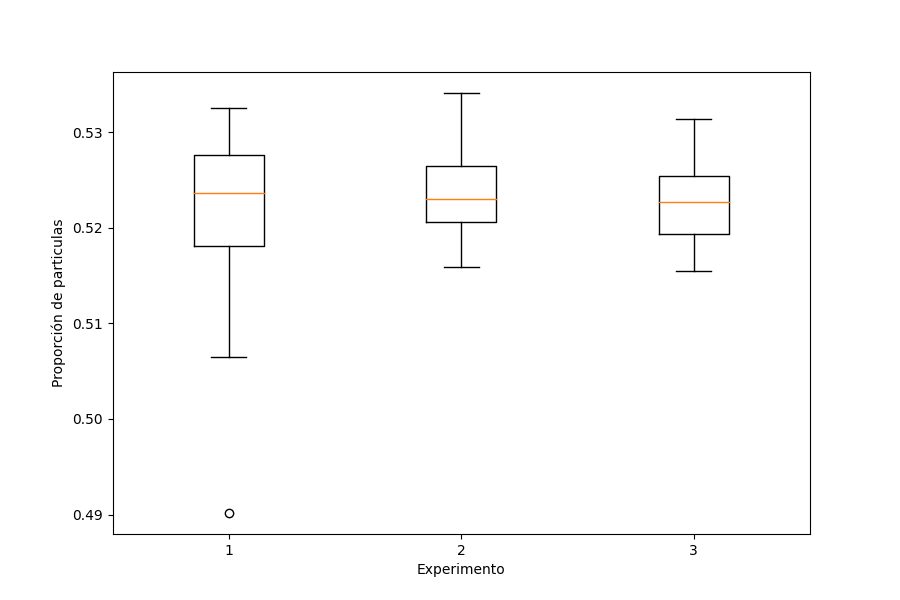
\includegraphics[width=0.5\linewidth]{bx_4.png}
	\caption{Proporción de particulas filtradas: k=10000,n=2000000}
	\label{fig:bx5}
	
	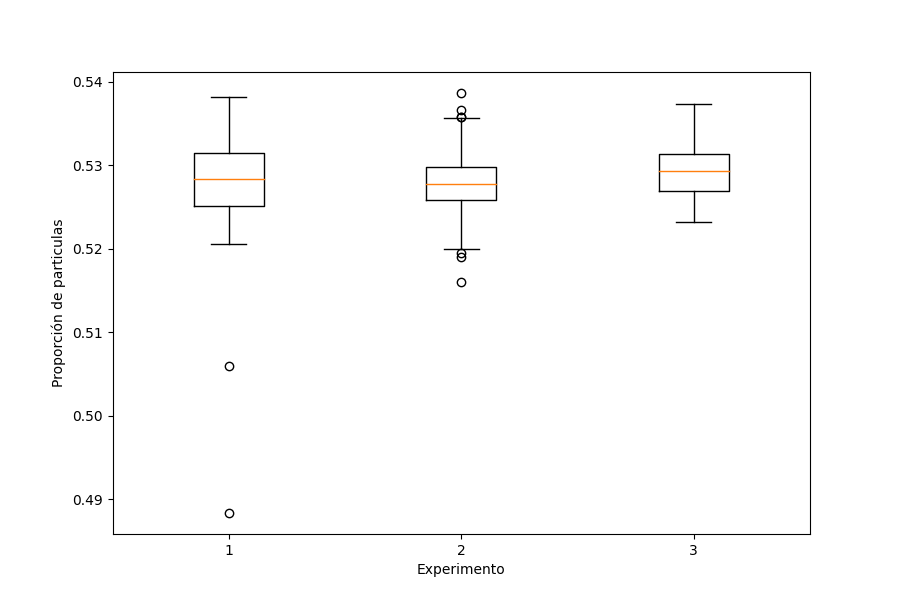
\includegraphics[width=0.5\linewidth]{bx_5.png}
	\caption{Proporción de particulas filtradas: k=10000,n=500000}
	\label{fig:bx6}
\end{figure}

	\section{Conclusiones}
	A continuación, se presentan las conclusiones basados en los resultados y el comportamiento de las variaciones de $k,n,t$.
	
	\begin{enumerate}
		\item  El tiempo de filtrado (t) parece no tener relevancia, la proporción de partículas filtradas parece muy estable en tiempos tempranos como en tiempos tardíos.
		\item Los valores de k,n parecen tampoco tener efecto sobre el proceso de filtrado, probablemente se deba a las funciones definidas para la unión o separación de cúmulos.
		
		
	\end{enumerate}

\bibliography{Biblio}
\bibliographystyle{plainnat}

\end{document}